% SI - Figure 1 Missing data
\begin{figure}[htb]
\centering
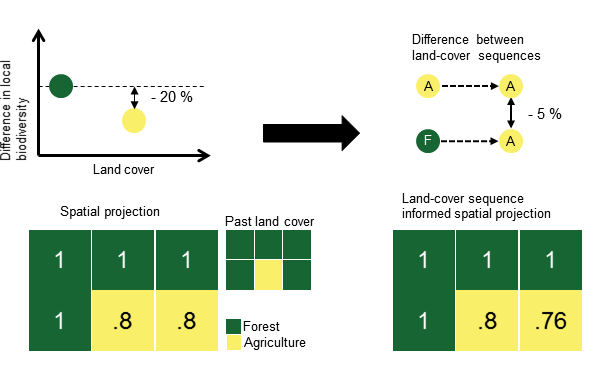
\includegraphics[width=1\textwidth]{chapter3/SI01}
\caption{ Average temporal distribution of Landsat data and an example times series of Landsat data. (\textbf{a}) Distribution of available Enhanced Vegetation Index (EVI) data in years covered by the Landsat missions. Points show the average monthly EVI data availability per year (0 to 12 months of data) across time series and PREDICTS sites grouped by 15\textdegree latitude bins. The size of points indicates the mean data availability (0 to 100\% with 100\% having 12 months of available data in a given year), while the colour shows the number of PREDICTS sites contributing to the mean (as PREDICTS sites were sampled in varying years). (\textbf{b}) Example time series for one PREDICTS site with a high proportion of missing data before 1999. In all analyses such time series were truncated to the period from 1999 onwards (indicated by the dashed line).}
\label{SI03_01}
\end{figure}

% SI - Figure 2 Binning
\begin{figure}[htb]
\centering
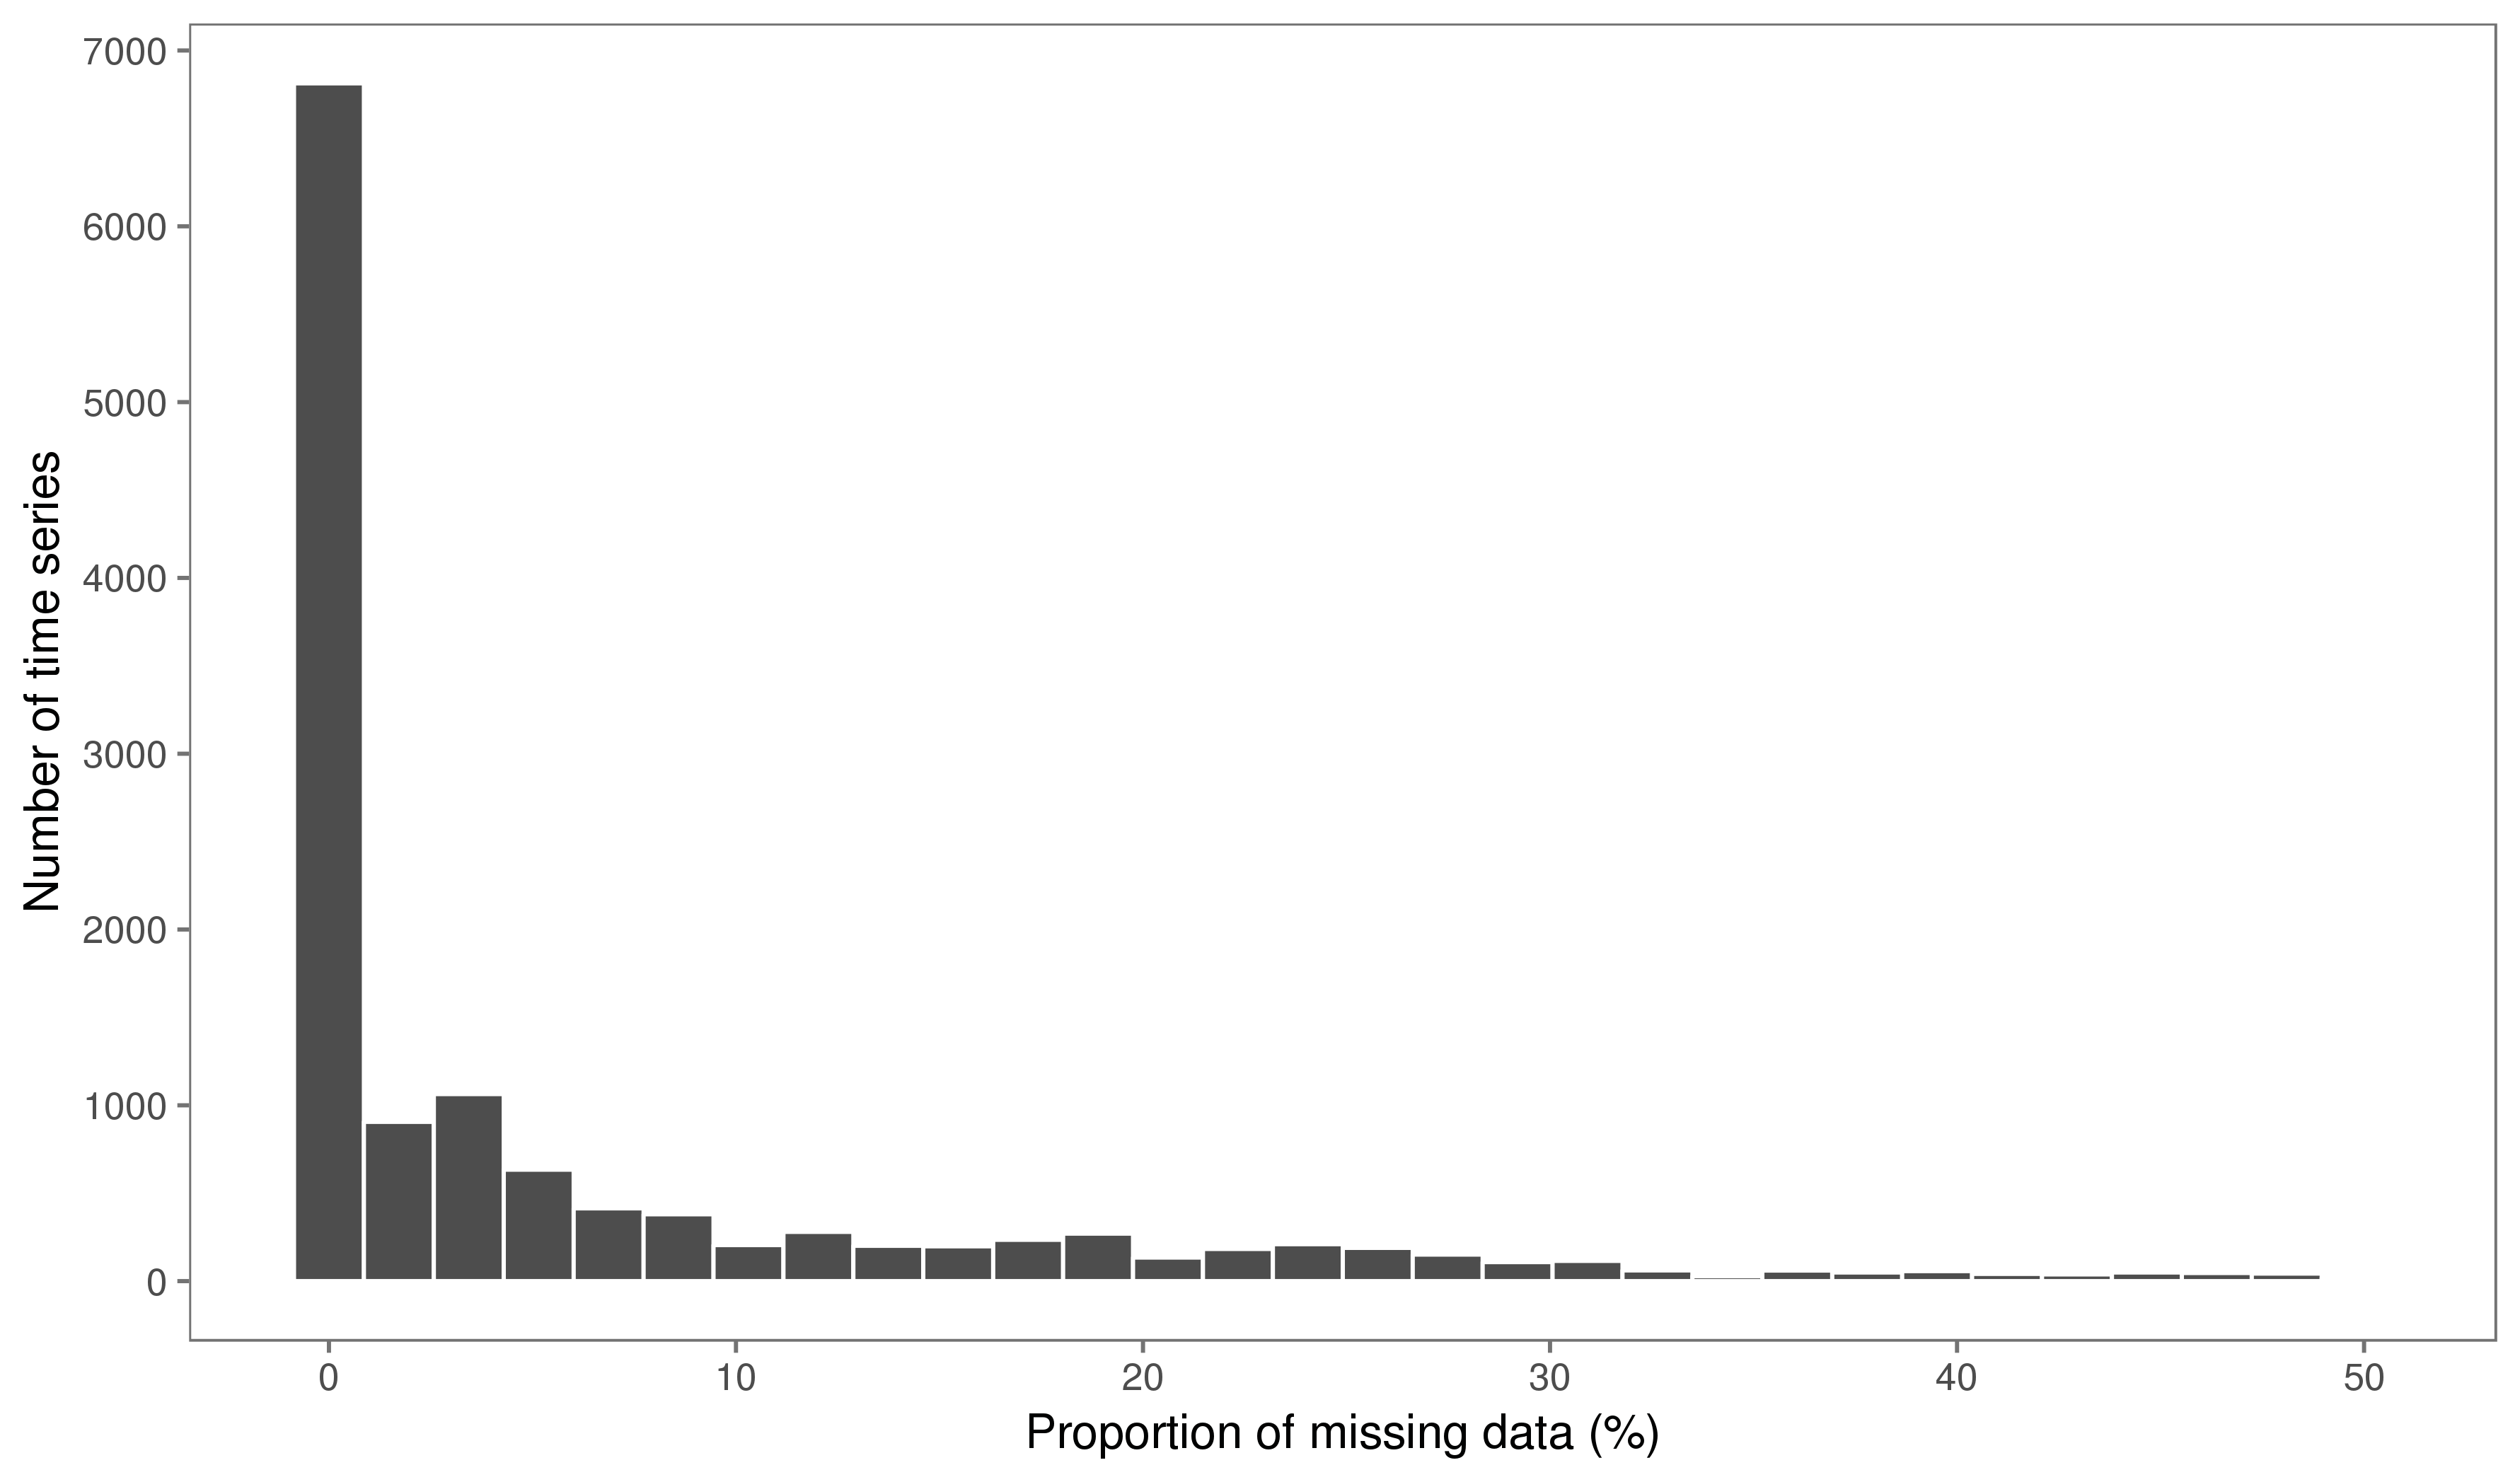
\includegraphics[width=1\textwidth]{chapter3/SI02}
\caption{ Number of sites with abrupt land change per attribute. Number of sites (black line) per attribute of abrupt land change with (\textbf{a}) the relative shift in magnitude, (\textbf{b}) the shift in trend as difference in annual EVI trend, and (\textbf{c}) the time passed between abrupt land change and biodiversity sampling. Background colours in (\textbf{a}) and (\textbf{b}) indicate the binning into six groups for shifts in magnitude (> 50\%, > 25\% to $\leq$ 50\%, and $\leq$ 25\% EVI loss [$---$ to $-$] or gain [$+++$ to $+$]), and in trend (0.01, 0.05, and > 0.05 annual negative [$---$ to $-$] to positive [$+++$ to $+$] EVI trend differences). Gray lines in (\textbf{c}) delineate bins of time passed ($\leq$ 5 years, > 5 and $\leq$ 10 years, and >10 years). Colours as in Figure \ref{F03_02}.}
\label{SI03_02}
\end{figure}

% SI Table 1------ %
% From here https://www.tablesgenerator.com/
\begin{table}[]
\centering
\caption{Number of PREDICTS sites and studies with an abrupt land change. Shown as either a change in magnitude (columns) and/or change in trend (trend). Symbols as in Figure \ref{F03_02}. }
\label{SIT03_01}
\begin{tabular}{@{}lllllllllll@{}}
                                          &                                           & \multicolumn{7}{c}{\textbf{Shift in magnitude}}                                                                                                                                                                    &                               &                             \\
                                          &                                           & \textbf{- - -}             & \textbf{- -}                & \textbf{-}                   & \textbf{0}                    & \textbf{+}                   & \textbf{+ +}                & \textbf{+ + +}              & \textbf{Total sites}          & \textbf{Studies}            \\ \cmidrule(l){3-11} 
                                          & \multicolumn{1}{l|}{- - -}                & 2                          & 8                           & 192                          & NA                            & 73                           & 26                          & 22                          & \cellcolor[HTML]{EFEFEF}323   & \cellcolor[HTML]{C0C0C0}57  \\
                                          & \multicolumn{1}{l|}{- -}                  & 7                          & 281                         & 642                          & NA                            & 497                          & 158                         & 53                          & \cellcolor[HTML]{EFEFEF}1638  & \cellcolor[HTML]{C0C0C0}175 \\
                                          & \multicolumn{1}{l|}{-}                    & 7                          & 88                          & 256                          & NA                            & 231                          & 154                         & 53                          & \cellcolor[HTML]{EFEFEF}789   & \cellcolor[HTML]{C0C0C0}184 \\
                                          & \multicolumn{1}{l|}{0}                    & NA                         & NA                          & NA                           & 10102                         & NA                           & NA                          & NA                          & \cellcolor[HTML]{EFEFEF}10102 & \cellcolor[HTML]{C0C0C0}358 \\
                                          & \multicolumn{1}{l|}{+}                    & 9                          & 102                         & 399                          & NA                            & 410                          & 205                         & 49                          & \cellcolor[HTML]{EFEFEF}1174  & \cellcolor[HTML]{C0C0C0}237 \\
                                          & \multicolumn{1}{l|}{\textbf{+ +}}         & 47                         & 172                         & 342                          & NA                            & 465                          & 254                         & 86                          & \cellcolor[HTML]{EFEFEF}1366  & \cellcolor[HTML]{C0C0C0}224 \\
\multirow{-7}{*}{\textbf{\rotatebox{90}{Shift in trend}}} & \multicolumn{1}{l|}{\textbf{+ + +}}       & 12                         & 137                         & 47                           & NA                            & 34                           & 12                          & 31                          & \cellcolor[HTML]{EFEFEF}273   & \cellcolor[HTML]{C0C0C0}56  \\
                                          & \multicolumn{1}{l|}{\textbf{Total sites}} & \cellcolor[HTML]{EFEFEF}84 & \cellcolor[HTML]{EFEFEF}788 & \cellcolor[HTML]{EFEFEF}1878 & \cellcolor[HTML]{EFEFEF}10102 & \cellcolor[HTML]{EFEFEF}1710 & \cellcolor[HTML]{EFEFEF}809 & \cellcolor[HTML]{EFEFEF}294 &                               &                             \\
                                          & \multicolumn{1}{c|}{\textbf{Studies}}     & \cellcolor[HTML]{C0C0C0}34 & \cellcolor[HTML]{C0C0C0}135 & \cellcolor[HTML]{C0C0C0}246  & \cellcolor[HTML]{C0C0C0}358   & \cellcolor[HTML]{C0C0C0}263  & \cellcolor[HTML]{C0C0C0}171 & \cellcolor[HTML]{C0C0C0}83  &                               &                            
\end{tabular}
\end{table}
% ------ %

% SI - Figure 3 Cross-correlations
\begin{figure}[htb]
\centering
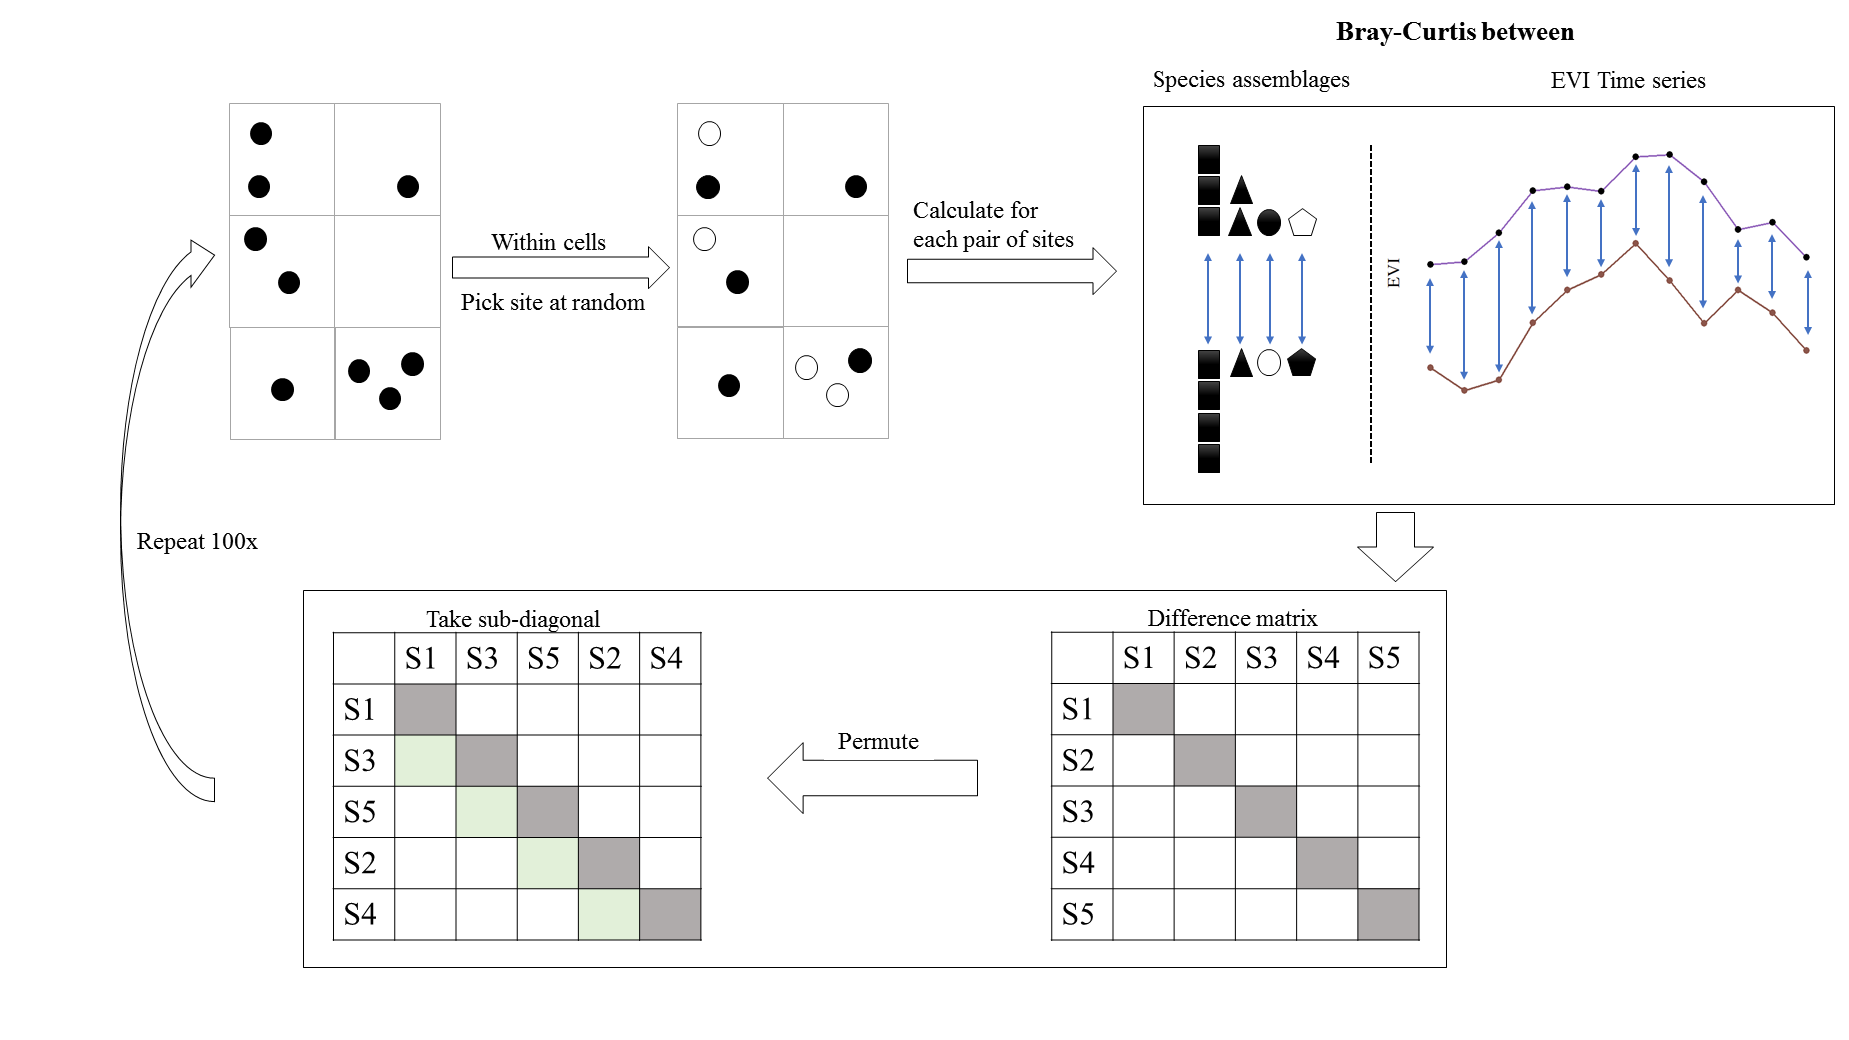
\includegraphics[width=1\textwidth]{chapter3/SI03}
\caption{ Correlations between attributes of abrupt land change. Showing shifts in magnitude, trend and time passed (see Methods). The lower facets show a point density plot, the upper facets the Pearson correlation coefficient between pairs of attributes and the diagonal a density plot.}
\label{SI03_03}
\end{figure}

% SI - Figure 4 violin plots
\begin{figure}[htb]
\centering
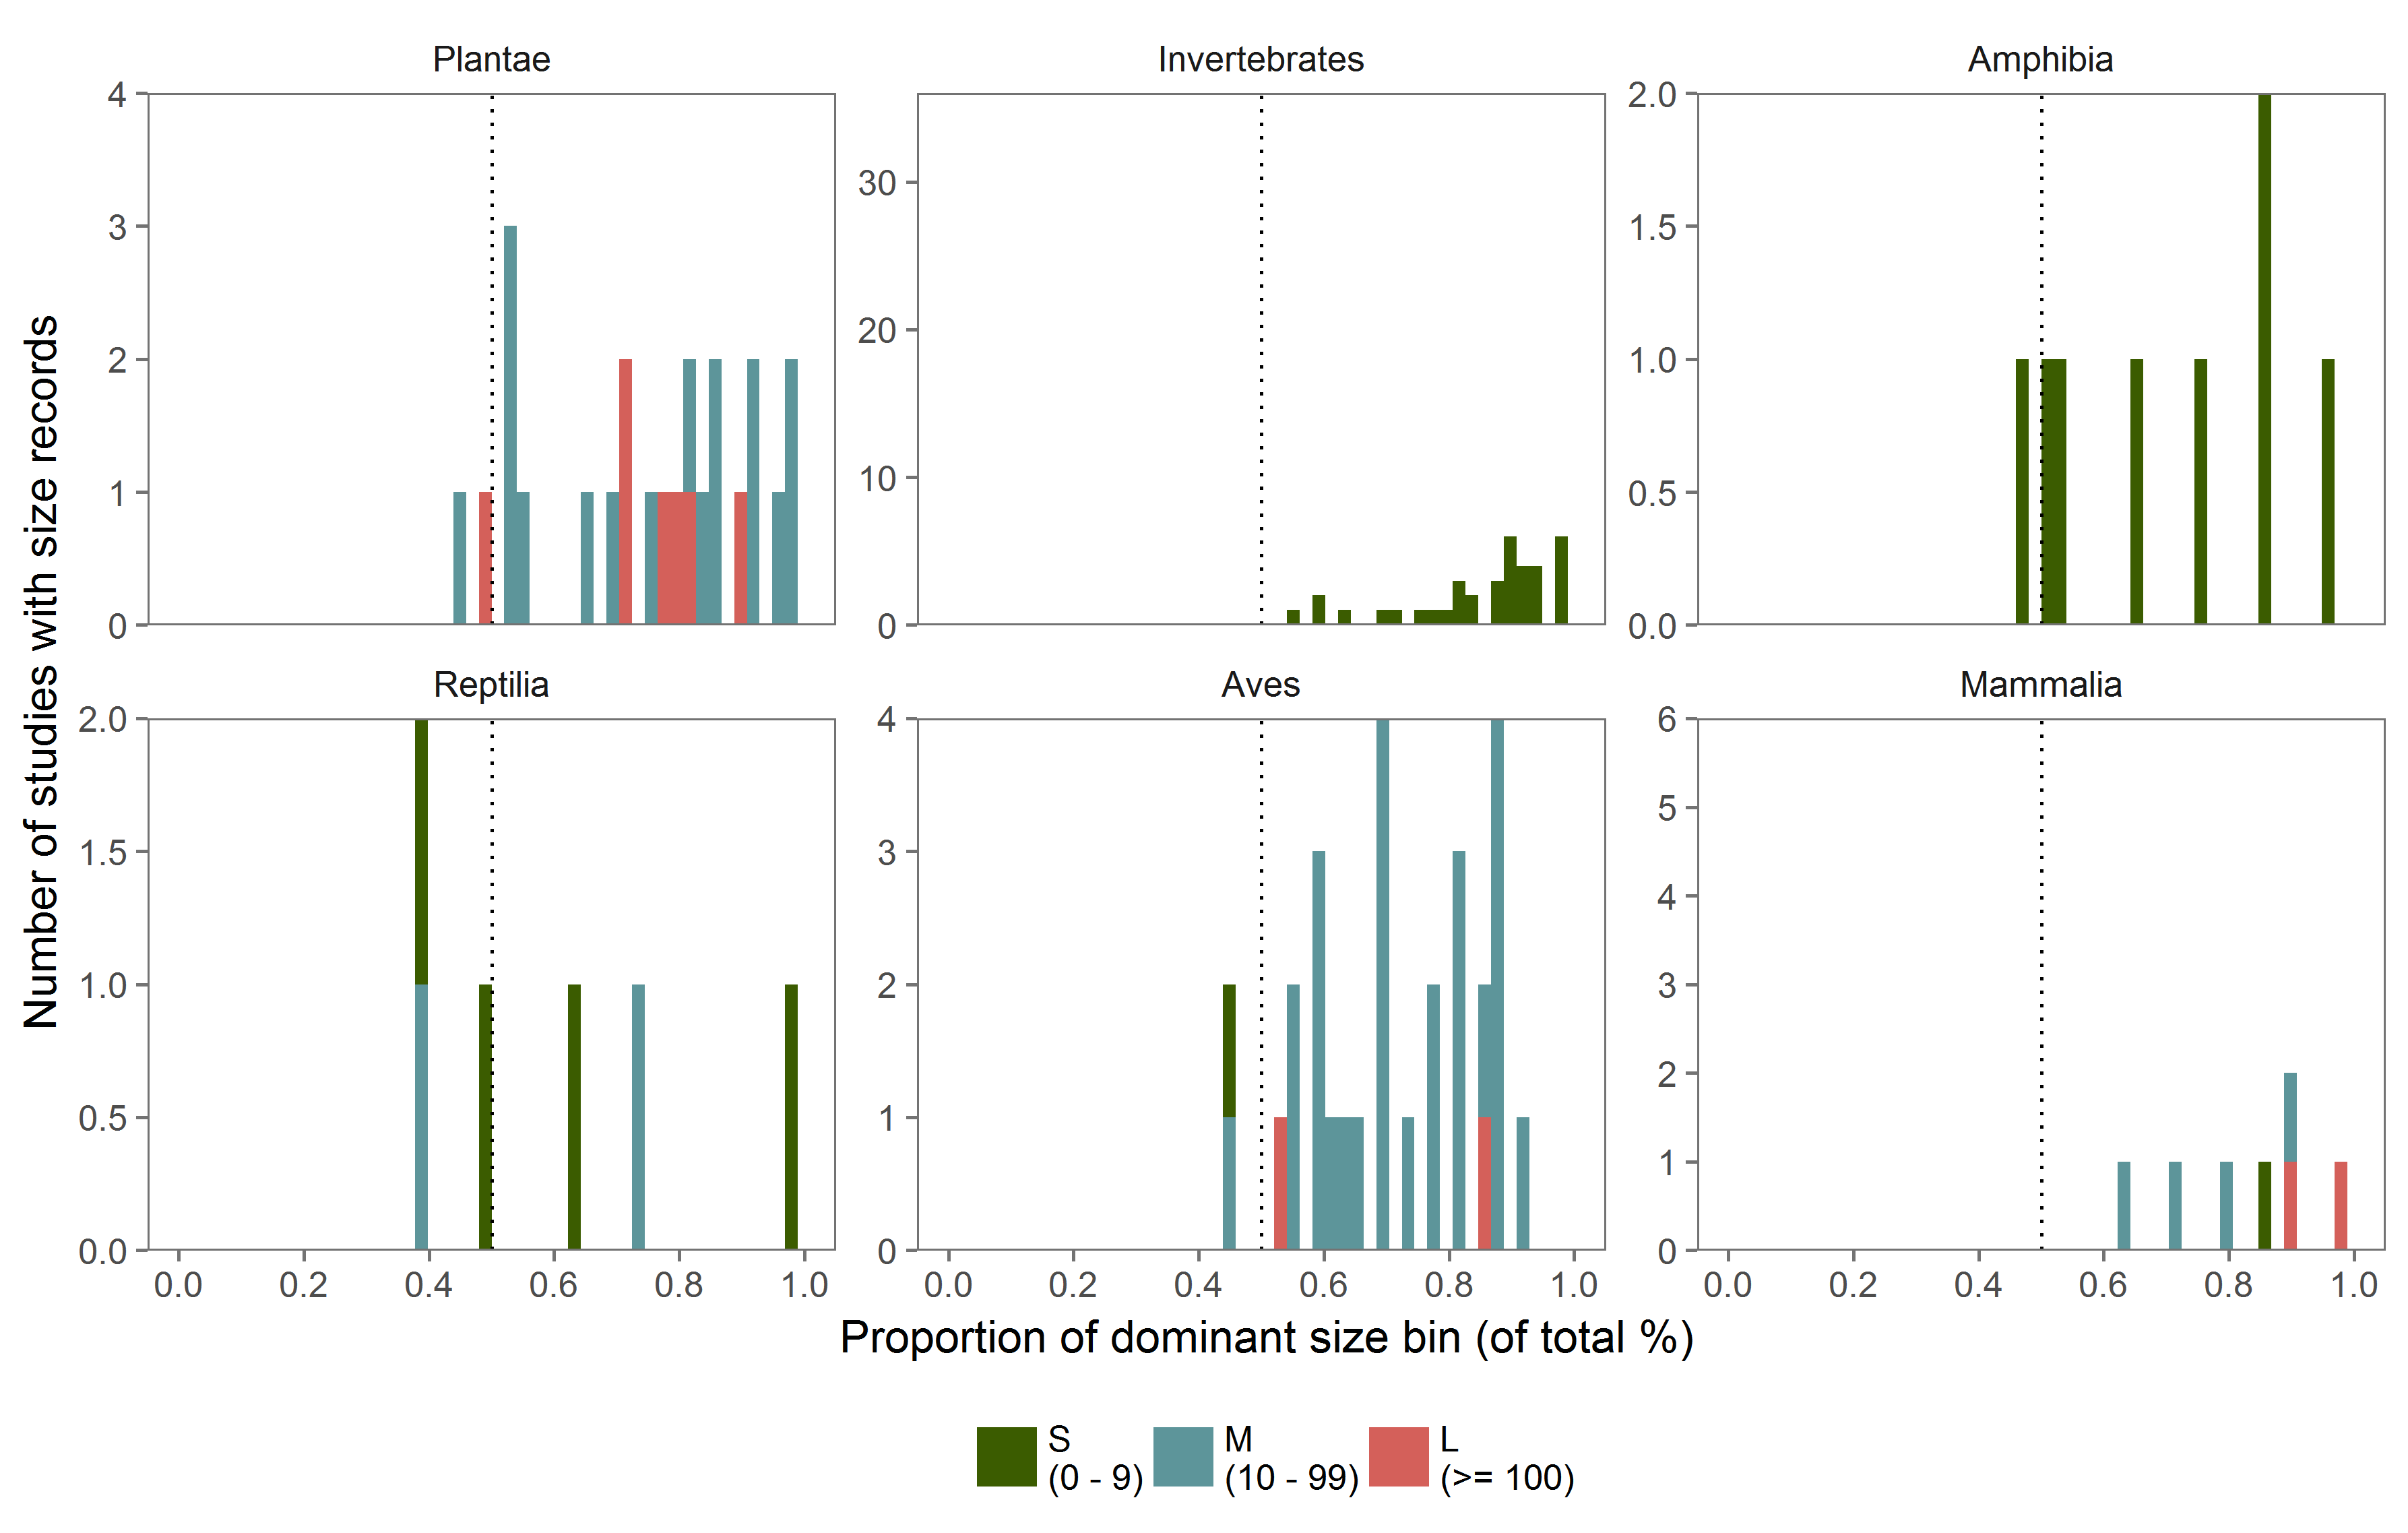
\includegraphics[width=1\textwidth]{chapter3/SI04}
\caption{ Distribution of time passed between abrupt land changes and start of biodiversity sampling. Shown for (\textbf{a}) shifts in magnitude, and (\textbf{b}) shift in trend bins. Colours as in Figure \ref{F03_02}. Black dots and error bars show the mean $\pm$ one standard deviation. Number of sampled sites per bin are shown above each bin.}
\label{SI03_04}
\end{figure}

% SI - Figure 5 Time dir version of figure 3
\begin{figure}[htb]
\centering
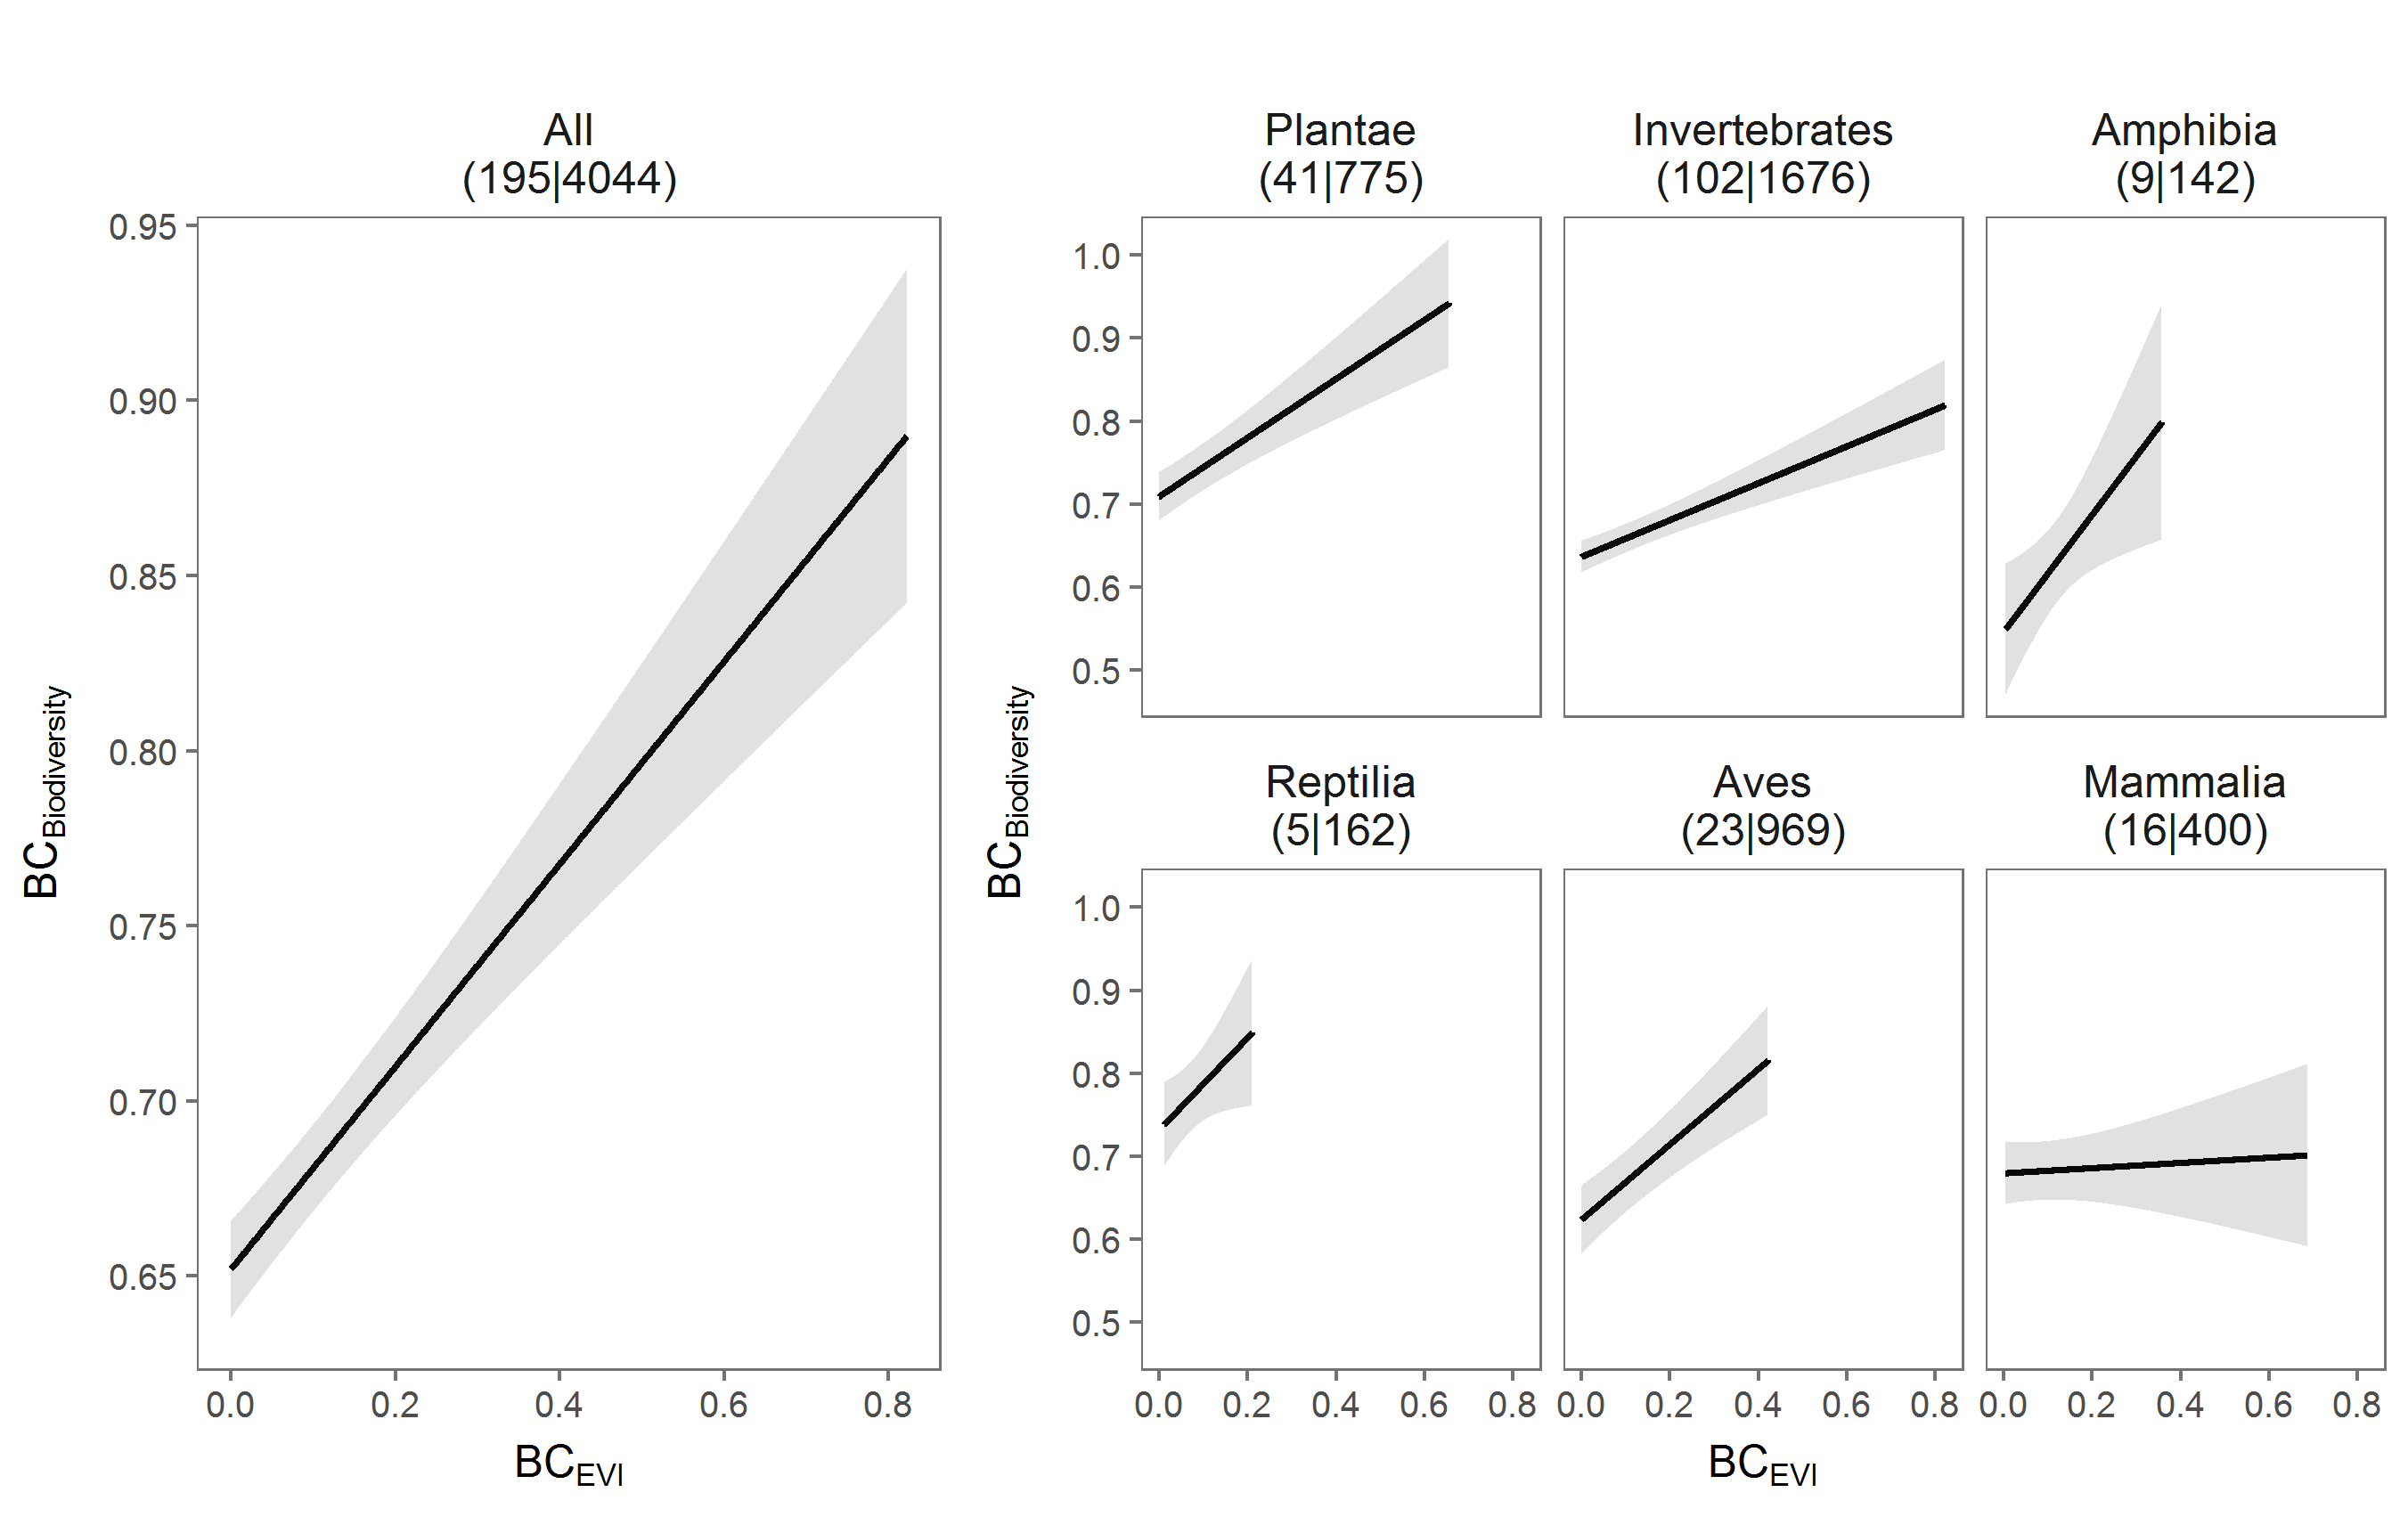
\includegraphics[scale = .8]{chapter3/SI05}
\caption{ Mean similarity in species assemblage composition (S\o rensen similarity index) between pairs of sites with a shift in trend. Calculated as average similarity within the same study and land-use category without (0) and with an abrupt land change with varying shifts in EVI trend (\textbf{a}). Colours indicate whether similarity of species assemblages was on average greater (purple) or smaller (brown) relative to unchanged sites. Symbols indicate positive ($+++$, $++$, $+$) or negative ($---$, $--$, $-$) shifts in trend of annual EVI (see Methods). Numbers in (\textbf{a}) indicate the total number of studies for which pairwise comparisons between sites could be made. (\textbf{b}) Dendrograms show hierarchical clustering of all pairwise similarities based on the average Manhattan distance between pairs of sites; sites with more similar assemblage composition are in branches of closer proximity. }
\label{SI03_05}
\end{figure}

\clearpage
